%! Author = TiagoRG
%! GitHub = https://github.com/TiagoRG

\chapter{Análise e Discussão}
\label{ch:analise-discussao}
{
%%%
% Conteúdo da Análise e Discussão aqui

\section{Parte A}
\label{sec:analise-discussao-parte1} 

\subsection{Resultados} \label{subsec:analise-discussao-parte1-resultados}
    Para o cálculo da constante de calibração, foi utilizada a montagem referida no enunciado, e registados os valores de $I_s$ e $V_H$.
    \par No gráfico abaixo é representada a reta de aproximação da função $V_h = f(I_s)$ , elaborada pelo software Excel com base nos dados obtidos experimentalmente.

\begin{figure}[h]
    \centering
    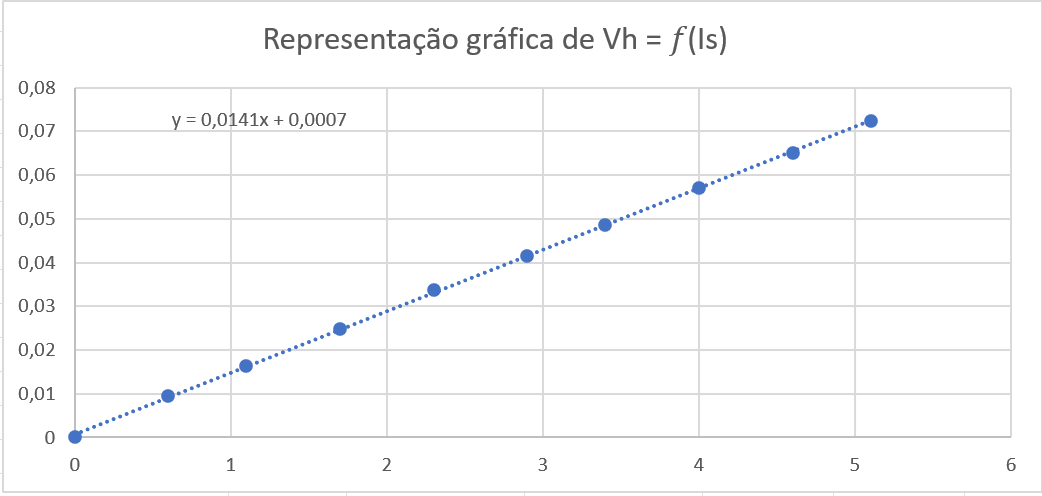
\includegraphics[scale=0.6]{images/grafico1-parte-a.png}
    \caption{Gráfico de representação linear de $I_s$ e $V_H$}
    \label{fig:grafico1-parte-a}
\end{figure}

    Na seguinte tabela, estão denotados os valores experimentais utilizados na elaboração do gráfico apresentado acima, e o valor calculado para a constante de calibração, $C_c$.

\begin{figure}[h]
    \centering
    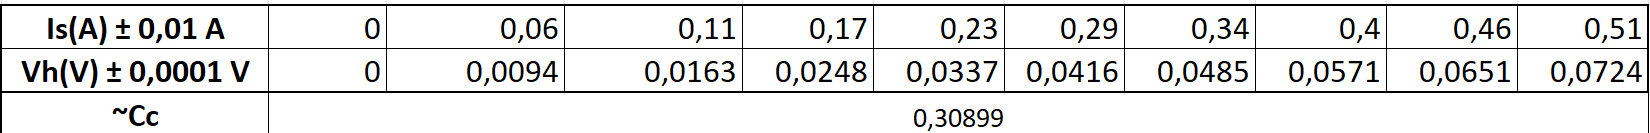
\includegraphics[scale=0.6]{images/tabela1-parte-a.png}
    \caption{Tabela de resultados (parte A)}
    \label{fig:tabela1-parte-a}
\end{figure}

\subsection{Análise} \label{subsec:analise-discussao-parte1-analise}
    Quanto aos resultados obtidos, o valor obtido de $C_c$ foi calculado usando a equação (5), e este tem um erro associado que foi calculado utilizando a equação (2). \ O desvio associado foi de $\Delta C_c = 2.03 \times 10^{-2}$.

\subsection{Discussão}
    Após as medições e cálculos efetuados, foi obtido o gráfico \ref{fig:grafico1-parte-a} e a equação da reta de aproximação cujos valores divergem minimamente dos medidos. \ O declive desta equação foi utilizado para o cálculo de $C_c$. 
    \par Como $\frac{N}{l}$ e $\mu_0$ são valores constantes, a única variável no cálculo de $C_c$ é apenas o declive da reta da função $f(I_s)$, que está relacionado com os valores medidos, logo estes são a única influência no erro.
    \par Estes erros podem ser, por exemplo, o erro associado aos instrumentos de medição, ou pequenas variações na calibração da sonda.
    
\pagebreak

\section{Parte B}
\label{sec:analise-discussao-parte2}

\subsection{Resultados}
\label{subsec:analise-discussao-parte2-resultados}
    Na parte B, foram efetuadas medições em 3 partes, repartidas em 3 tabelas e gráficos. \ Estas representam a variação dos campos magnéticos gerados pelas bobines, consoante a posição da sonda de Hall.
    \par Na tabela 1, apenas a bobine imóvel tem corrente elétrica. \ Na tabela 2, apenas a bobine móvel tem corrente elétrica. \ Na tabela 3, as duas bobines estão ligadas em série, ambas com a mesma corrente elétrica. 
    \par Estas tabelas estão representadas na figura abaixo. 

    \begin{figure}[H]
        \centering
        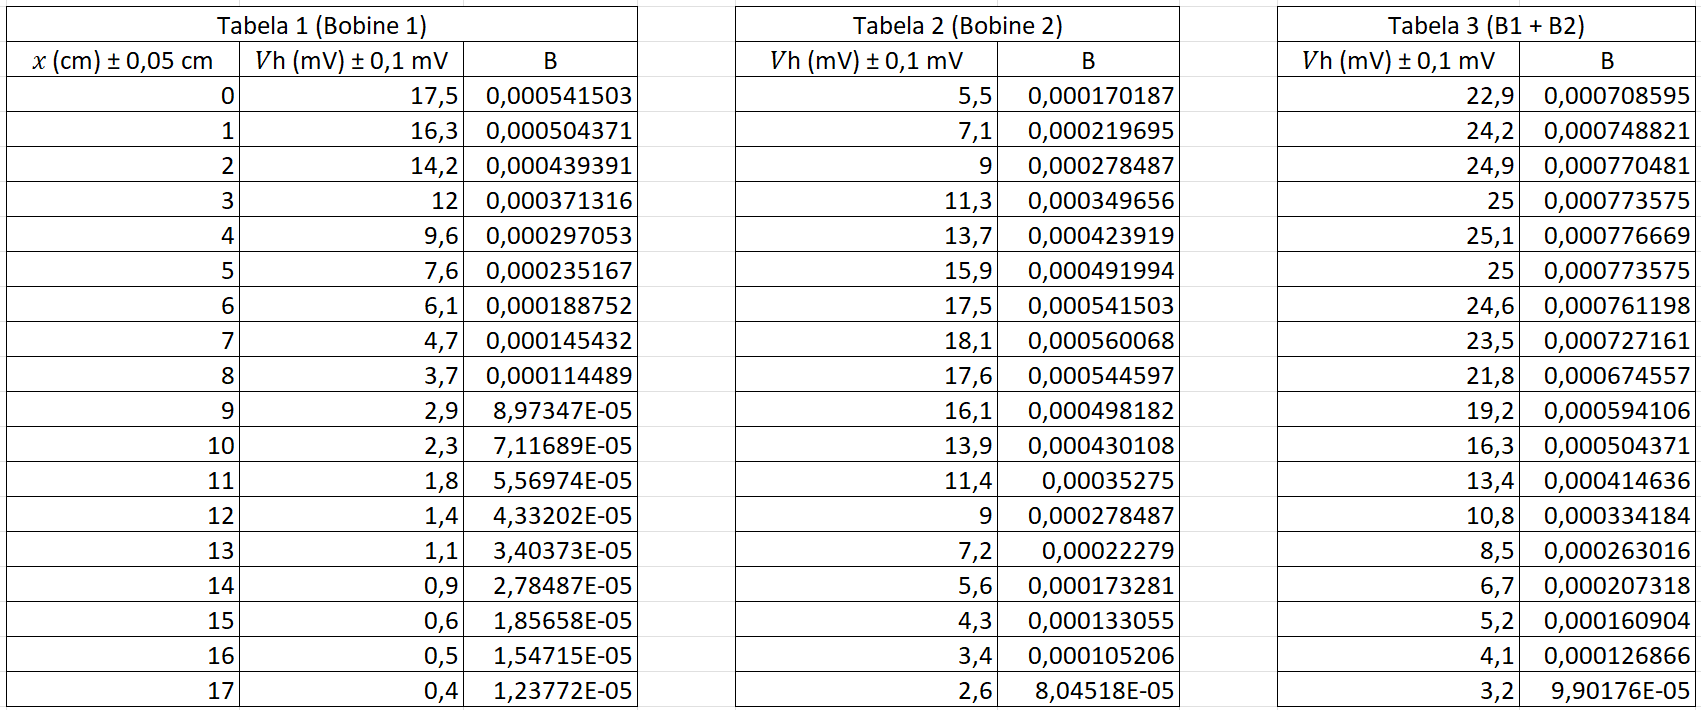
\includegraphics[scale=0.6]{images/tabelas1-3-parte-b.png}
        \caption{Tabelas representativas dos campos magnéticos}
    \end{figure}

    Em baixo está representado os gráficos das respetivas tabelas em função à posição da sonda de Hall.

    \begin{figure}[H]
        \centering
        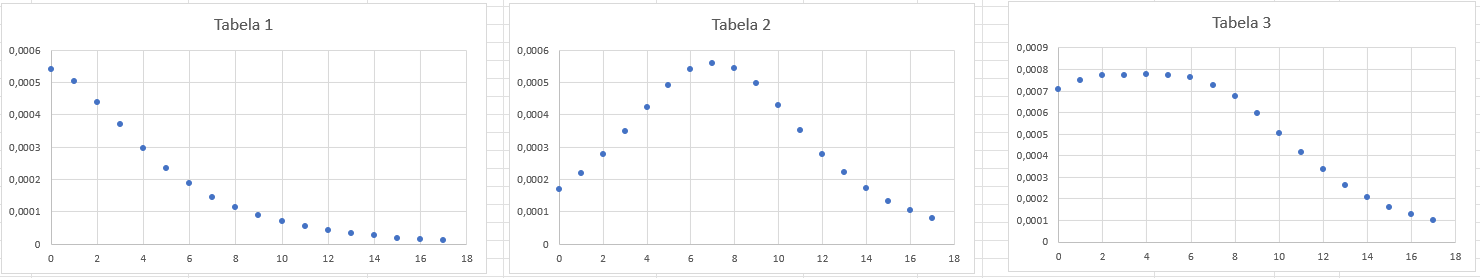
\includegraphics[scale=0.6]{images/graficos1-3-parte-b.png}
        \caption{Gráficos representativos das tabelas}
    \end{figure}

\subsection{Análise}
\label{subsec:analise-discussao-parte2-analise}
    O Princípio da Sobreposição do campo magnético consiste em que, numa configuração de Helmholtz, a soma do valor dos campos individualmente gerados numa dada posição da sonda de Hall será igual ao valor medido com as duas bobines ativas.

    \par Ao observar os resultados obtidos, a propriedade fundamental do Princípio da Sobreposição verifica-se de forma aproximada, ou seja, embora a soma dos campos individualmente medidos não seja exatamente igual ao valor medido aquando da medição simultânea dos dois campos, os valores são próximos.

    \par Nos gráficos está apresentado de forma mais clara este princípio. \ Com isto, podemos afirmar que ocorre sobreposição dos campos magnéticos.
    
    \par Para estimar o nº de espiras, foi utilizada a equação (4) para calcular o campo magnético no eixo de um anel de corrente. \ Após obter o resultado do campo magnético,  utiliza-se o $B_{max}$ obtido na tabela 3, usando a equação (6).


\subsection{Discussão}
\label{subsec:analise-discussao-parte2-discussao}
    Dado por completo os cálculos necessários, e a análise dos resultados obtidos, e a discrepância entre os valores teóricos e práticos, para a verificação do Princípio da Sobreposição do campo magnético. \ Estes desvios são originados por margens de erro, nos valores que este está dependente, como a constante de calibração e as medições da diferença de potencial numa dada posição.

    \par No cálculo do nº de espiras, o erro associado à estimativa deve-se a diversos fatores, como os erros associados ao cálculo do valor máximo obtido no campo magnético, e o cálculo de $B(x)$.

%%%
}
